\documentclass{report}
\usepackage[utf8]{inputenc}
\usepackage[T1]{fontenc}
\usepackage{CormorantGaramond}
\usepackage{fontspec}
\usepackage{geometry}
\usepackage[table]{xcolor}
\usepackage{tabularx}
\usepackage{graphicx}
\usepackage{mathtools}
\usepackage[bottom]{footmisc}
\usepackage[italian]{babel}
\usepackage{hyperref}
\usepackage{titlesec}
\usepackage{listings}
\usepackage{color}
\usepackage{graphicx}
\usepackage{fancyhdr}
\usepackage{float}

\graphicspath{{contenuti/images}}

\renewcommand{\headrulewidth}{0.4pt}
\renewcommand{\footrulewidth}{0.4pt}

\lstset{ % General setup for the package
    basicstyle=\small\sffamily,
    numbers=left,
     numberstyle=\tiny,
    frame=tb,
    tabsize=4,
    columns=fixed,
    showstringspaces=false,
    showtabs=false,
    keepspaces,
    commentstyle=\color{red},
    keywordstyle=\color{blue}
}

\geometry{
a4paper,
total = {170mm, 240mm},
left = 20mm,
top = 20mm,
}

\setlength{\headheight}{33.60004pt}

\setlength{\parindent}{0em}
\setlength{\parskip}{0.7em}

\titlespacing*{\section}{0pt}{0.7em}{0.5em}
\titlespacing*{\subsection}{0pt}{0.7em}{0.5em}

\newcommand{\gassets}{../}



\renewcommand{\title}{
    PoC
    
    \tiny Versione documento: \textit{V0.0.1}
}

\newcommand{\people}{
    \normalsize
    \begin{center}
        \begin{tabularx}{7cm}{l | X}            
            \textbf{Uso} & Esterno\\
            \textbf{Destinatario} & Committente\\
            & Cliente \\
        \end{tabularx}
    \end{center}
}

\fancypagestyle{plain}{%
    \fancyhead{} % clear all header fields
    \fancyhead[L]{\leftmark}
    \fancyhead[R]{\textit{SWEasabi} \includegraphics[height=30pt]{\gassets global-assets/img/loghi/SWEasabi_compact_logo.png}}
    \fancyfoot{} % clear all footer fields
    \fancyfoot[L]{\thepage}
    \fancyfoot[R]{Piano di qualifica}
}

\begin{document}

\pagestyle{fancy}

\fancyhead{} % clear all header fields
\fancyhead[L]{\leftmark}
\fancyhead[R]{\textit{SWEasabi} \includegraphics[height=30pt]{\gassets global-assets/img/loghi/SWEasabi_compact_logo.png}}
\fancyfoot{} % clear all footer fields
\fancyfoot[L]{\thepage}
\fancyfoot[R]{Piano di qualifica}


\input{\gassets global-assets/tex/header}
\thispagestyle{empty}
\clearpage
%\pagenumbering{Roman}
%\section{Registro delle modifiche}

%Tabella
\begin{center}
    \begin{tabularx}{\linewidth}{|l|l|X|X|}            
        \hline
        \textbf{Versione} & \textbf{Data} & \textbf{Modifica}& \textbf{Persone}\\
        \vzerozerotre
        \vzerozerodue
        \vzerozerouno
        \hline

    \end{tabularx}
\end{center}

\tableofcontents
\clearpage
\pagenumbering{arabic}
\chapter{Tecnologie}\label{tecnologie}

\begin{itemize}
    \item Angular
    \item Java Spring
    \item mqtt
    \item Java
\end{itemize}
\chapter{Scopo}\label{scopo}

Lo scopo del POC è quello di dimostrare padronanza di una limitata selezione di tecnologie rilevanti al progetto. In particolare, le principali tecnologie utilizzate sono state Angular per la pagina front-end, Java Spring per l'api REST e Mosquitto come broker mqtt.

\begin{figure}
    
\includegraphics[width=\linewidth]{poc.jpg}
    \caption{Simple visual representation}
\end{figure}
\chapter{API Java Spring}\label{funzionamento}

\section{Introduzione}

Lo scopo dell'API è quello di fornire servizi REST alla pagina angular e comunicare con le applicazioni che vanno a svolgere la logica effettiva del progetto. In particolare, vengono offerte due GET (rispettivamente disponibili su Lamps e Lamps/id) e una PUT (anch'essa su Lamps/id). Nel progetto sarà presente un'ulteriore separazione tra API e servizi in modo da non esporli all'esterno (con l'API che si occuperà di verificare che la richiesta avvenga da un utente autorizzato e dirigendola verso la corretta applicazione), tuttavia essendo questo PoC puramente a scopo dimostrativo questa feature non è qui presente in quanto l'enfasi è stata posta sulla corretta comunicazione tra le diverse parti del progetto, ritenendo il processo di autenticazione vero e proprio superfluo in questo PoC (come confermato dal committente).

\section{Funzionamento}

\subsection{Database}

Per migliorare il funzionamento del PoC, è stato dotato di un piccolo database temporaneo a cui viene fatto un preload di alcune variabili durante l'inizializzazione del programma.

\subsection{Richieste GET}

Il progetto offre due GET, una su lamps e una su lamps/id. Queste GET ritornano rispettivamente i dettagli di tutte le lampade presenti (ad esempio il loro id, dove sono situate, o il loro status, ovvero se si tratta di una lampadina accesa o spenta) o quelli di una singola lampada corrispondente all'id selezionato.

\begin{figure}[H]
    \centering
    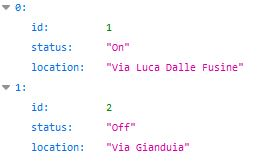
\includegraphics{lamps.jpg}
    \caption{Api risponde a richiesta su /Lamps}
\end{figure}

\begin{figure}[H]
    \centering
    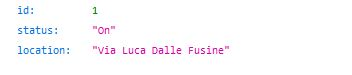
\includegraphics{lampsid.jpg}
    \caption{Api risponde a richiesta su /Lamps/1}
\end{figure}

\subsection{Richiesta PUT}

Come menzionato sopra il progetto offre anche una PUT, anch'essa a Lamps/id. Questo servizio consente di modificare i dettagli della lampadina corrispondente, in particolare di modificare il proprio stato (quindi accenderla o spegnerla).

\begin{figure}[H]
    \centering
    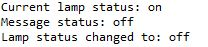
\includegraphics{put1.jpg}
    \caption{Richiesta PUT: La lampadina non è nello stato richiesto}
\end{figure}

\begin{figure}[H]
    \centering
    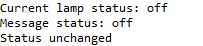
\includegraphics{put2.jpg}
    \caption{Richiesta PUT: La lampadina è già nello stato richiesto}
\end{figure}

\subsection{Comunicazione MQTT}

A ogni richiesta effettuata, l'API posta messaggi sui topic relativi alle lampadine utilizzando mqtt (nel caso del nostro progetto con broker mosquitto), messaggi che vengono successivamente letti dalle nostre applicazioni in back-end. Come spiegato sopra, questo passaggio è essenziale in quanto serve a comunicare con i servizi veri e propri facendogli eseguire le diverse operazioni richieste, tuttavia è più a scopo dimostrativo sul funzionamento della comunicazioni in questo PoC.

\begin{figure}[H]
    \centering
    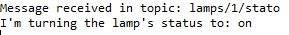
\includegraphics{mqtt.jpg}
    \caption{Richiesta PUT: Client legge il messaggio mqtt in arrivo dall'API}
\end{figure}
\chapter{Angular}\label{angular}

\section{Introduzione}

La pagina Angular mostra due differenti bottoni , uno di Fetch dello stato della API e un altro che modifica lo stato dell'entitá\footnote{nel dominio del POC la prima entitá ID=0} , in questo bottone di modifica,il comportamento é quello di fetchare lo stato della lampada,per poi modificarlo nel suo complementare.

\end{document}
